\documentclass[11pt,table]{beamer}
\mode<presentation>
\usepackage{etex}
\usepackage{graphicx}
\usepackage{epstopdf}
\usepackage[english]{babel}
\usepackage{tabularx}
\usepackage{booktabs}
\usepackage{mathrsfs}
\usepackage{multicol}
\usepackage{bm}
\usepackage{subcaption}
\usepackage{wrapfig}
\usepackage{dcolumn}
\usepackage{threeparttable}
\usepackage{booktabs}
\usepackage{bbm}
\usepackage{amsmath,dsfont,listings}
\usepackage{amssymb}
\usepackage{rotating}
\usepackage{multirow}
\usepackage{tcolorbox}
\usepackage[authoryear]{natbib}
\usepackage{circledsteps}
\usepackage{qtree}

\usepackage{tikz}
\usetikzlibrary{arrows,decorations.pathmorphing,backgrounds,fit,positioning,shapes.symbols,chains, shapes}
\setbeamertemplate{section in toc}[sections numbered]
\setbeamertemplate{caption}[numbered]

\bibliographystyle{Econometrica}

\setbeamersize{text margin right=3.5mm, text margin left=7.5mm}  % text margin
\setbeamersize{sidebar width left=0cm, sidebar width right=0mm}
\setbeamertemplate{sidebar right}{}
\setbeamertemplate{sidebar left}{}

\definecolor{text-grey}{rgb}{0.45, 0.45, 0.45} % grey text on white background
\definecolor{bg-grey}{rgb}{0.66, 0.65, 0.60} % grey background (for white text)
\definecolor{fu-blue}{RGB}{0, 51, 102} % blue text
\definecolor{fu-green}{RGB}{153, 204, 0} % green text
\definecolor{fu-red}{RGB}{204, 0, 0} % red text (used by \alert)
\definecolor{BrewerBlue}{HTML}{377EB8} % Define Brewer Blue
\definecolor{BrewerRed}{HTML}{E41A1C}  % Define Brewer Red
\definecolor{BlueD}{HTML}{496a93}
\definecolor{BlueF}{HTML}{b9cde5}

\setbeamertemplate{frametitle}{%
    \vskip-30pt \color{text-grey}\large%
    \begin{minipage}[b][23pt]{\textwidth}%
    \flushleft\insertframetitle%
    \end{minipage}%
}

\setbeamertemplate{navigation symbols}{} 

%%% begin title page
\setbeamertemplate{title page}{
\vskip2pt\hfill
\vskip19pt\hskip3pt

% set the title and the author
\vskip4pt
\parbox[top][1.35cm][c]{11cm}{\LARGE\color{text-grey} \textcolor{red1}{RL}earning:\\[1ex] \inserttitle \\[1ex] \small \quad \\[3ex]}
\vskip17pt
\parbox[top][1.35cm][c]{11cm}{\small Unit 4-2: \insertsubtitle \\[2ex] \insertauthor \\[1ex]}
}
%%% end title page

%%% colors
\usecolortheme{lily}
\setbeamercolor*{normal text}{fg=black,bg=white}
\setbeamercolor*{alerted text}{fg=fu-red}
\setbeamercolor*{example text}{fg=fu-green}
\setbeamercolor*{structure}{fg=fu-blue}

\setbeamercolor*{block title}{fg=white,bg=black!50}
\setbeamercolor*{block title alerted}{fg=white,bg=black!50}
\setbeamercolor*{block title example}{fg=white,bg=black!50}

\setbeamercolor*{block body}{bg=black!10}
\setbeamercolor*{block body alerted}{bg=black!10}
\setbeamercolor*{block body example}{bg=black!10}

\setbeamercolor{bibliography entry author}{fg=fu-blue}
\setbeamercolor{bibliography entry journal}{fg=text-grey}
\setbeamercolor{item}{fg=fu-blue}
\setbeamercolor{navigation symbols}{fg=text-grey,bg=bg-grey}
%%% end colors

%%% headline
\setbeamertemplate{headline}{
\vskip30pt
}
%%% end headline

%%% footline
\newcommand{\footlinetext}{
%\insertshortinstitute, \insertshorttitle, \insertshortdate
}
\setbeamertemplate{footline}{
\vskip2pt
\hfill \raisebox{-1pt}{\usebeamertemplate***{navigation symbols}}
\hfill \insertframenumber\hspace{10pt}
\vskip4pt
}
%%% end footline

%%% settings for listings package
\lstset{extendedchars=true, showstringspaces=false, basicstyle=\footnotesize\sffamily, tabsize=2, breaklines=true, breakindent=10pt, frame=l, columns=fullflexible}
\lstset{language=Java} % this sets the syntax highlighting
\lstset{mathescape=true} % this switches on $...$ substitution in code
% enables UTF-8 in source code:
\lstset{literate={ä}{{\"a}}1 {ö}{{\"o}}1 {ü}{{\"u}}1 {Ä}{{\"A}}1 {Ö}{{\"O}}1 {Ü}{{\"U}}1 {ß}{\ss}1}
%%% end listings

\usepackage{concmath}
\usepackage{xcolor}
\definecolor{red1}{RGB}{206, 17, 38}
\definecolor{blue1}{RGB}{16, 118, 208}
\definecolor{gray1}{RGB}{117, 115, 115}
\usepackage{hyperref}


\newtheorem{proposition}{Proposition}
\newtheorem{assumption}{Definition}

\title[]{Short guides to reinforcement learning}
\subtitle[]{Deep Neural Networks}
\author[D. Rostam-Afschar]{\textcolor{gray1}{Davud Rostam-Afschar (Uni Mannheim)}}
\date[]{\today}
\subject{Econometrics}
\renewcommand{\footlinetext}{\insertshortinstitute, \insertshorttitle, \insertshortdate}
\hypersetup{
    bookmarks=false,
    unicode=false,
    pdftoolbar=false,
    pdffitwindow=true,
    pdftitle={Reinforcement Learning for Business, Economics, and Social Sciences: \insertsubtitle},
    pdfauthor={Davud Rostam-Afschar},
    pdfsubject={Reinforcement Learning},
    pdfkeywords={reinforcement learning, Deep Neural Networks},
    pdfnewwindow=true,
}
\def\sym#1{\ifmmode^{#1}\else\(^{#1}\)\fi}

\begin{document}

\begin{frame}[plain]
  \titlepage
\end{frame}

% --------------------------------------------------- Slide --
%\begin{frame}
	%\frametitle{Content}
	%\tableofcontents[]
%\end{frame}

\section{Deep Neural Networks}
{
\setbeamercolor{background canvas}{bg=BrewerBlue}
\begin{frame}
\centering
\Huge
\textcolor{white}{How to improve flexibility of approximation?}
\thispagestyle{empty}
\end{frame}
}


{
\setbeamercolor{background canvas}{bg=BrewerBlue}
\begin{frame}
\centering
\Huge
\textcolor{white}{Deep Neural Networks}
\thispagestyle{empty}
\end{frame}
}


\begin{frame}{Deep Neural Networks}


\begin{itemize}
    \item Definition: neural network with \textcolor{teal}{many} hidden layers

\item Advantage: \textcolor{teal}{high expressivity}
 \item Challenges:
\begin{itemize}
    \item \textcolor{red1}{How should we train a deep neural network?}
\item \textcolor{red1}{How can we avoid overfitting?}
 
\end{itemize}
    
   
\end{itemize}
    \citep{goodfellow2016deep}    

\end{frame}

\begin{frame}{Mixture of Gaussians}
\begin{columns}[T]
\begin{column}{0.5\textwidth}

\begin{itemize}
    \item Shallow neural network  (flat mixture)
 
\end{itemize}
\scalebox{0.65}{
\centering
\begin{tikzpicture}[x=50pt,y=50pt,
        N/.style={draw=BlueD,fill=BlueF,line width=1pt,inner sep=0pt,align=center},
        OP/.style={circle,N,text width=14pt},
        GI/.style={ellipse,N,text width=32pt},
        R/.style={N,rectangle,text width=220pt,minimum height=20pt},
        D/.style={BlueD},
        Idn/.style={midway,font=\footnotesize,fill=white,inner sep=0.75pt},
    ]
    \node[GI,text width=50pt,minimum height=30pt] (Id) at (3,3) {Identity};
    %
    \node[R,anchor=south] (I) at (Id.north) {Output};
    %
    \node[R] (I) at (3,1) {Inputs};
    %
    %
    \foreach \n in {1,2,3,4,5} {
        \node[GI] (G\n) at (\n,1.8) {Gauss ian};
        \draw (Id)--(G\n) node[Idn]{$1/k$};
        \draw (G\n.south)--(G\n.south|-I.north);
    }
    %
    \node[above] at (G1.north) {Hidden layer};
\end{tikzpicture}
}
\end{column}
\begin{column}{0.5\textwidth}
\uncover<2->{
\begin{itemize}
    \item Deep neural network  (hierarchical mixture)
 
\end{itemize}

\scalebox{0.65}{
\begin{tikzpicture}[x=50pt,y=30pt,
        N/.style={draw=BlueD,fill=BlueF,line width=1pt,inner sep=0pt,align=center},
        OP/.style={circle,N,text width=14pt},
        GI/.style={ellipse,N,text width=32pt},
        R/.style={N,rectangle,text width=180pt,minimum height=20pt},
        D/.style={BlueD},
    ]
    %
    \node[OP] (l1) at (1.5,5) {$+$};
    \node[OP] (l2) at (1.5,4) {$*$};
    \node[OP] (l3) at (1.5,3) {$+$};
    %
    \node[OP] (r1) at (3.5,5) {$+$};
    \node[OP] (r2) at (3.5,4) {$*$};
    \node[OP] (r3) at (3.5,3) {$+$};
    %
    \foreach \n in {1,2,3,4} {\node[GI] (G\n) at (\n,2) {Gauss ian};}
    %
    \node[R] (I) at (2.5,1) {Inputs};
    %
    \foreach \n [remember=\n as \nprev (initially 1)] in {2,3} {
        \draw[D] (l\nprev)--(r\n);
        \draw[D] (r\nprev)--(l\n);
        \foreach \lr in {l,r} {\draw[D] (\lr\nprev.south)--(\lr\n.north);}
    }
    %
    \foreach \lr in {l} {\foreach \GI in {1,2} {\draw[D] (\lr3)--(G\GI);}}
    \foreach \lr in {r} {\foreach \GI in {3,4} {\draw[D] (\lr3)--(G\GI);}}
    \foreach \GI in {1,2,3,4} {\draw[D] (G\GI.south)--(G\GI.south|-I.north);}
\end{tikzpicture}
}
}
\uncover<3>{Sum-Product Network

(Exponentially large mixture of Gaussians but linear hierachy)
}
\end{column}
\end{columns}
    
\end{frame}

\begin{frame}{Image Classification}
    \begin{itemize}
        \item ImageNet Large Scale Visual Recognition Challenge
 
    \end{itemize}
    \vspace{3mm}
\begin{center}
    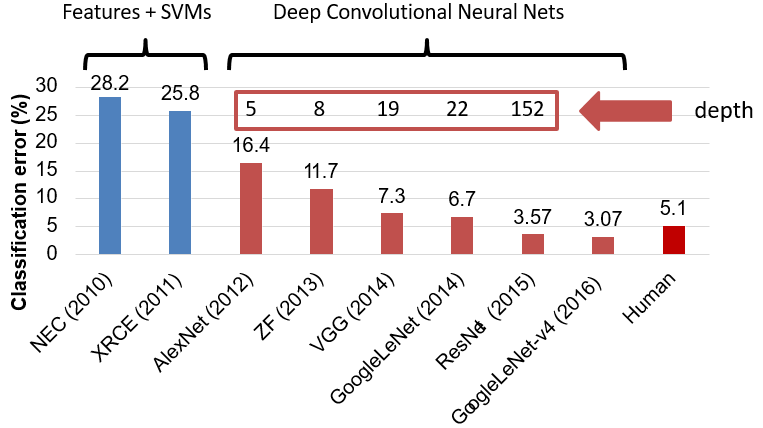
\includegraphics[width=0.9\textwidth]{figures/12.PNG}
\end{center}

\end{frame}

\section{Vanishing Gradients}
{
\setbeamercolor{background canvas}{bg=BrewerBlue}
\begin{frame}
\centering
\Huge
\textcolor{white}{Vanishing Gradients}
\thispagestyle{empty}
\end{frame}
}
\begin{frame}{Vanishing Gradients}


   \begin{itemize}
       \item Deep neural networks of sigmoid and  hyperbolic units often suffer from vanishing  gradients 
   \end{itemize} 

\vspace{3mm}
\begin{center}
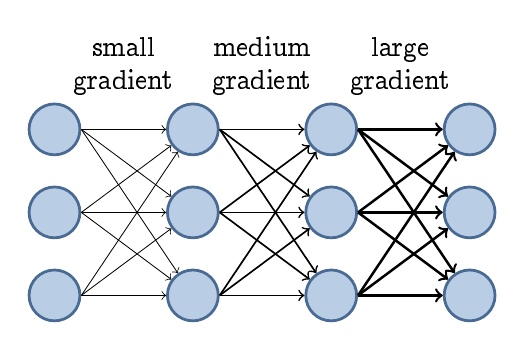
\begin{tikzpicture}[x=50pt,y=30pt,
        N/.style={circle,draw=BlueD,fill=BlueF,line width=1pt,inner sep=0pt,align=center},
        BN/.style={N,text width=14pt},
        G/.style={->},
        G2/.style={G,line width=0.3pt},
        G3/.style={G,line width=0.6pt},
        G4/.style={G,line width=0.9pt},
        L/.style={above,align=center},
    ]
    %
    \foreach \col in {1,2,3,4} {
        \foreach \row in {1,2,3} {
            \node[BN] (Nc\col r\row) at (\col,\row) {\strut};
        }
    }
    %
    \foreach \col [remember=\col as \colprev (initially 1)] in {2,3,4} {
        \foreach \row in {1,2,3} {
            \foreach \rownext in {1,2,3} {
                \draw[G\col] (Nc\colprev r\row.east)--(Nc\col r\rownext);
            }
        }
    }
    %
    \foreach \leg [count=\pos] in {small,medium,large} {\node[L] at ({\pos+0.5},3.3) {\leg\\ gradient};}
\end{tikzpicture}
\end{center}
   
\end{frame}

\begin{frame}{Sigmoid and hyperbolic units}


\begin{itemize}
    \item Derivative is always less than 1
 
\end{itemize}
    \vspace{3mm}
\begin{center}
    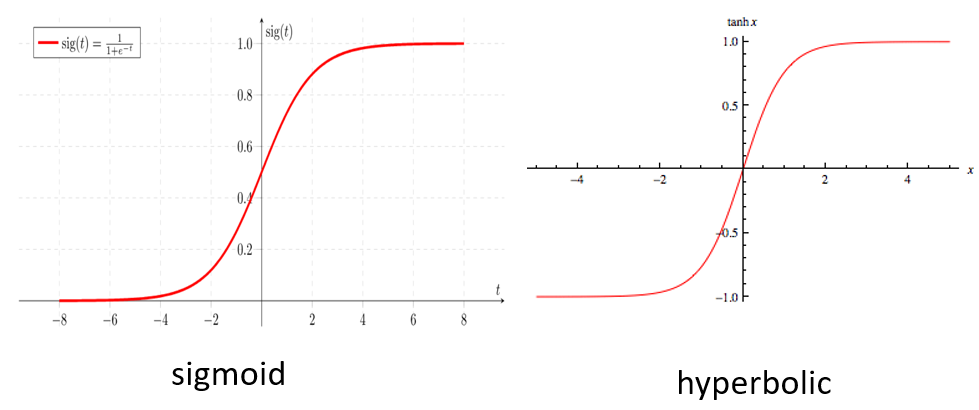
\includegraphics[width=1\textwidth]{figures/14.PNG}
\end{center}
\end{frame}

\begin{frame}{Simple Example}
\small
\begin{itemize}
    \item  $y=\sigma\Biggl(w_{4} \sigma\biggl(w_{3} \sigma\Bigl(w_{2} \sigma\bigl(w_{1} x\bigr)\Bigr)\biggr)\Biggr)$ 

\begin{center}
\begin{tikzpicture}[x=50pt,y=30pt,
    N/.style={circle,draw=BlueD,fill=BlueF,line width=1pt,inner sep=0pt,align=center},
    BN/.style={N,text width=14pt},
    E/.style={->,line width=0.9pt},  % default, will be overridden
    En/.style={midway,above,font=\footnotesize,inner sep=1pt},
]
  % nodes
  \foreach \n [count=\pos] in {{x},{h_1},{h_2},{h_3},{y}} {
    \node[BN] (N\pos) at (\pos,0) {$\n$};
  }

  % edges with vanishing widths
  \foreach [count=\i from 1] \e [remember=\e as \eprev (initially 1)] in {2,3,4,5} {
    % compute width = 0.9pt - 0.3pt * i
		\edef\lw{\dimexpr 0.3pt*\i\relax}
    \draw[E, line width=\lw]
      (N\eprev.east) -- (N\e.west)
      node[En] {$w_\eprev$};
  }
\end{tikzpicture}

\end{center}

\item Common weight initialization in (-1,1)
\item Sigmoid function and its derivative always less than 1
\item This leads to vanishing gradients:

$$
\begin{aligned}
& \frac{\partial y}{\partial w_{4}}=\sigma^{\prime}\left(a_{4}\right) \sigma\left(a_{3}\right) \\
& \frac{\partial y}{\partial w_{3}}=\sigma^{\prime}\left(a_{4}\right) w_{4} \sigma^{\prime}\left(a_{3}\right) \sigma\left(a_{2}\right) \leq \frac{\partial y}{\partial w_{4}} \\
& \frac{\partial y}{\partial w_{2}}=\sigma^{\prime}\left(a_{4}\right) w_{4} \sigma^{\prime}\left(a_{3}\right) w_{3} \sigma^{\prime}\left(a_{2}\right) \sigma\left(a_{1}\right) \leq \frac{\partial y}{\partial w_{3}} \\
& \frac{\partial y}{\partial w_{1}}=\sigma^{\prime}\left(a_{4}\right) w_{4} \sigma^{\prime}\left(a_{3}\right) w_{3} \sigma^{\prime}\left(a_{2}\right) w_{2} \sigma^{\prime}\left(a_{1}\right) x \leq \frac{\partial y}{\partial w_{2}}
\end{aligned}
$$
    
\end{itemize}
    
\end{frame}

\begin{frame}{Mitigating Vanishing Gradients}


\begin{itemize}
    \item Some popular solutions:
\begin{itemize}
    \item Pre-training
\item \textbf{Rectified linear units}
\item Batch normalization
\item Skip connections
 
\end{itemize} 
\end{itemize}
    
\end{frame}

\begin{frame}{Rectified Linear Units}
    \begin{itemize}
        \item Rectified linear: $h(a)=\max (0, a)$
        \begin{itemize}
            \item Gradient is 0 or 1
\item Sparse computation
 
        \end{itemize}

\uncover<2->{
\begin{columns}[T]
\begin{column}{0.4\textwidth}
\begin{itemize}
    \item Soft version

(``Softplus''):

$h(a)=\log \left(1+e^{a}\right)$ 
\end{itemize}
\end{column}
\begin{column}{0.6\textwidth}
\centering
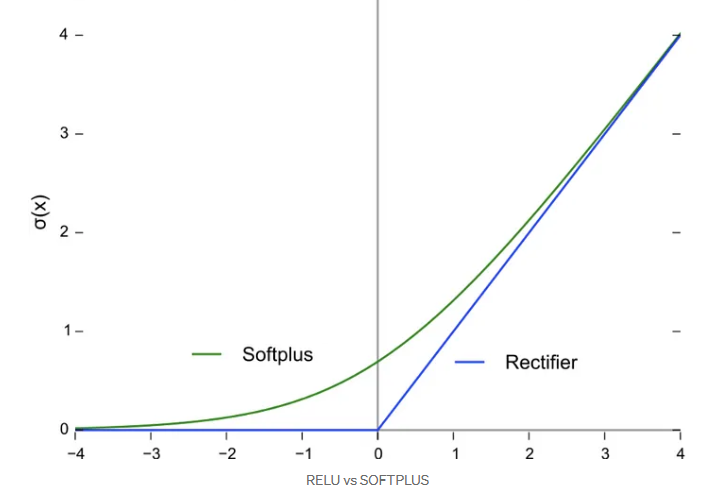
\includegraphics[width=0.8\textwidth]{figures/16.png}
\end{column}
\end{columns}
}
\uncover<3>{
\item \textcolor{red1}{Warning: softplus does not prevent gradient vanishing}\\ (gradient $<1$ ) 
}        
    \end{itemize}
\end{frame}


\begin{frame}[t,allowframebreaks
]%\nocite{*}
\frametitle{References}
\small
\bibliography{bib}
\end{frame}
\section{Takeaways}
{
\setbeamercolor{background canvas}{bg=BrewerBlue}
\begin{frame}
\centering
\Huge
\textcolor{white}{Takeaways}
\thispagestyle{empty}
\end{frame}
}

\begin{frame}{How do Deep Neural Networks Help Modeling Complex Data?}

\begin{itemize}
    \item Use multiple hidden layers
    \item They enable complex function approximation
    \item A key challenge is the vanishing gradient problem
    \item Solutions include ReLU activation functions, batch normalization, skip connections, and pre-training
    \item Rectified Linear Units (ReLU) help mitigate vanishing gradients 
\end{itemize}
\end{frame}


\end{document}
